\chapter[Diseño del observador del estado para estimación de fuerzas]{Diseño del observador del estado para estimación de fuerzas externas.}
\label{chap:disenoObservador}

A lo largo del presente capítulo se describe el algoritmo de estimación propuesto, partiendo del modelo del sistema real, cuyos resultados pueden consultarse en el próximo capítulo. Posteriormente se mostrarán diversos aspectos que es necesario mencionar acerca de la puesta en práctica del algoritmo desarrollado para efectuar la estimación de fuerzas externas así como para el acondicionamiento de datos y la verificación de la observabilidad. \par 

El algoritmo presentado y el procedimiento seguido se ha basado en el desarrollado en \cite{garcia2008sensor}, pero introduciendo ciertas modificaciones para el cumplimiento de las leyes físicas que rigen el comportamiento del sistema. \par 

\newpage
\section{Introducción}

Como se ha explicado en el presente texto, para la estimación de la fuerza externa aplicada a la herramienta del robot se dispone de la información proveniente de dos sensores, a saber: sensor fuerza-par situado en la muñeca, y un sensor inercial (\acrshort{imu}). Combinando la información proveniente de dichos sensores, se presenta a continuación un método para efectuar esta estimación.\par

En la fuerza y momento medidos por el sensor fuerza par, se incluyen distintas componentes, debidas a la gravedad, a la inercia del extremo del robot y a la interacción del robot con el entorno. Un modelo en el que se consideren todas ellas es, por tanto, fundamental para una correcta estimación de las fuerzas externas, y cancelación de las demás.\par

El desarrollo del algoritmo propuesto se ha basado en el uso de un Filtro de Kalman Extendido para efectuar la fusión sensorial necesaria para combinar la información proveniente de las distintas fuentes de las que se dispone, como son el sensor fuerza-par situado en la muñeca del brazo robótico y el sensor inercial.\par

Es preciso en primer lugar modelar el sistema representado por el extremo del robot, considerando únicamente la herramienta Robotiq, el sensor fuerza-par de ATI Industrial, situado en la muñeca, y el sensor inercial. Para ello se ha de partir del comportamiento dinámico del sistema en cuestión, descrito mediante las ecuaciones de Newton-Euler. \par

\section{Consideraciones previas}

Un visión esquemática del sistema real puede verse en la siguiente figura \ref{fig:esquemasistema}. Los sistemas de referencia asociados a cada elemento se especifican a continuación:

\begin{itemize}
  \item $\{S_P\}$, sistema de referencia asociado al centro de masas, cuyos ejes $X_P$, $Y_P$, $Z_P$, coinciden con los ejes principales de inercia de la herramienta.
  \item $\{S_S\}$, sistema de referencia asociado al sensor fuerza-par.
  \item $\{S_I\}$, sistema de referencia asociado al sensor inercial.
  \item $\{S_W\}$, sistema de referencia fijo, asociado a la base del robot.
  \item $\{S_E\}$, sistema de referencia ligado al punto de aplicación de la fuerza externa.
\end{itemize}

\begin{figure}[h!]
\centering
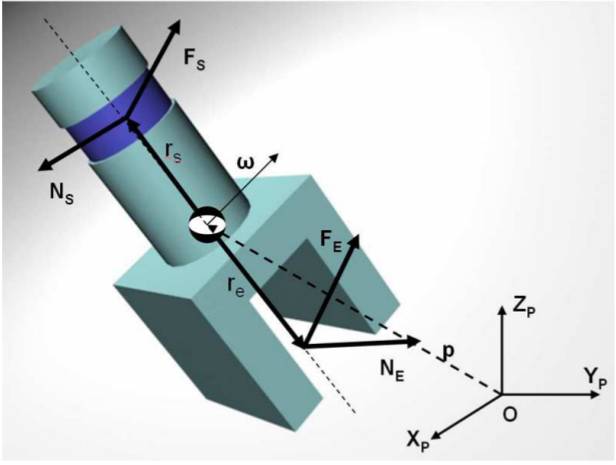
\includegraphics[scale=0.6]{Figuras/EsquemaSistema}
\caption[Visión esquemática del sistema considerado, con fuerzas y sistemas de referencia]{Visión esquemática del sistema considerado, en el que se incluyen las distintas fuerzas aplicables al mismo, así como ciertos sistemas de referencia considerados.}
\label{fig:esquemasistema}
\end{figure}

Para expresar las fuerzas y momentos, a lo largo del capítulo se empleará una notación compacta, que facilitará el tratamiento de esta información. Mediante esta notación, las fuerzas y momentos se agrupan en un mismo vector, de manera que:

\[
	\boldsymbol{U} = 
	\begin{pmatrix} 
		\boldsymbol{F} \\ \boldsymbol{N} 
	\end{pmatrix}
\] \par

Para realizar un cambio de sistema de referencia, de una fuerza medida en $A$ a la misma expresada en $B$, siguiendo la notación definida en \cite{sciavicco2000modelling}, se empleará la siguiente expresión, en la que $\boldsymbol{^Br_A}$ representa el vector posición desde $B$ hasta $A$ expresado en la base de $B$, ${^BR_A}$ es la matriz de cambio de base del sistema $A$ al $B$:

\begin{equation}
	\boldsymbol{U_B} = 
	\begin{pmatrix} 
		\boldsymbol{F_B} \\ \boldsymbol{N_B} 
	\end{pmatrix} = 
	\begin{pmatrix}
		{^BR_A} & 0_{3\times3} \\ S(\boldsymbol{^Br_A}){^BR_A} & {^BR_A}
	\end{pmatrix}
	\begin{pmatrix} 
		\boldsymbol{F_A} \\ \boldsymbol{N_A} 
	\end{pmatrix} =
	{^BT_A} \boldsymbol{U_A}
\label{eq:cambiowrench}
\end{equation} 

En esta última expresión (\ref{eq:cambiowrench}), se ha hecho uso del operador $S(.)$, el cual representa un producto vectorial en forma matricial, por ejemplo, siendo $r$ y $q$ dos vectores cualesquiera, se define el operador $S(.)$ como se muestra a continuación:

\[ 
 	\boldsymbol{r} \times \boldsymbol{q} = S(\boldsymbol{r})\boldsymbol{q} = 
  	\begin{pmatrix}
		0 & -r_3 & r_2 \\ r_3 & 0 & -r_1 \\ -r_2 & r_1 & 0
	\end{pmatrix}
	\begin{pmatrix}
		q_1 \\ q_2 \\ q_3
	\end{pmatrix}
\]

\section{Modelado del sistema real}

Considérese un sólido rígido, de masa $m$, con matriz de inercia $\boldsymbol{I}_{cm}$, expresada con respecto al sistema de referencia $\{S_P\}$ ligado a su centro de masas, el sistema queda modelado mediante las siguientes ecuaciones, donde $1_{3\times3}$ representa la matriz identidad de orden 3:

\begin{equation}
	\begin{pmatrix}
		\boldsymbol{F} \\ \boldsymbol{N}
	\end{pmatrix}
	=
	\begin{pmatrix}
		m1_{3\times3} & 0_{3\times3} \\ 0_{3\times3} & \boldsymbol{I}_{cm}
	\end{pmatrix}
	\begin{pmatrix}
		\boldsymbol{a}_p \\ \boldsymbol{\alpha}
	\end{pmatrix} +
	\begin{pmatrix}
		0_{3\times3} \\ \boldsymbol{\omega} \times \boldsymbol{I}\boldsymbol{\omega}
	\end{pmatrix}
\label{eq:newtoneuler}	
\end{equation}

Se ha propuesto un modelo del sistema en variables de estado, puesto que permite la estimación de la evolución temporal del estado del sistema, así como de las medidas de los sensores en cuestión. \par 

En el caso más general, como ya se ha mencionado con anterioridad, los sistemas dinámicos diferenciales pueden ser representados por un modelo de estado compuesto por dos expresiones:

\begin{subequations}
\begin{align}
	\boldsymbol{\dot{x}}(t) = f(\boldsymbol{x}(t),\boldsymbol{u}(t),t)
	\label{eq:ecestado} \\
	\boldsymbol{y}(t) = h(\boldsymbol{x}(t),\boldsymbol{u}(t),t)
	\label{eq:ecsalida}
\end{align}
\end{subequations} \\
\noindent
de las cuales (\ref{eq:ecestado}) recibe el nombre de \emph{ecuación de estado} y define la evolución temporal del estado del sistema, y (\ref{eq:ecsalida}) es denominada como \emph{ecuación de salida} y relaciona el estado del sistema con los datos de los sensores. \par

La formulación del modelo de estado del sistema se basa en la ecuación de Newton-Euler descrita en (\ref{eq:newtoneuler}), para ello es preciso definir el vector de estado $\boldsymbol{x}$, el vector de salida $\boldsymbol{y}$, y entradas $\boldsymbol{U}_S$, $\boldsymbol{U}_E$ y $\boldsymbol{U}_G$, tal y como se muestra a continuación:

\begin{equation}
\begin{split}
	[\boldsymbol{x}] &= [\boldsymbol{p}^T,\boldsymbol{q}^T,\boldsymbol{v}_p^T,\boldsymbol{\omega}^T]^T \in \Re^{13} \\
	[\boldsymbol{y}] &= [\boldsymbol{p}^T,\boldsymbol{q}^T,\boldsymbol{F_S}^T,\boldsymbol{N_S}^T,\boldsymbol{\omega}^T,\boldsymbol{a}_p^T,\dot{\boldsymbol{\omega}}^T]^T \in \Re^{22} \\
	[\boldsymbol{U}_S] &= [\boldsymbol{F}_S^T, \boldsymbol{N}_S^T]^T \in \Re^{6} \\
	[\boldsymbol{U}_E] &= [\boldsymbol{F}_E^T, \boldsymbol{N}_E^T]^T \in \Re^{6} \\
	[\boldsymbol{U}_G] &= [\boldsymbol{g}] \in \Re^{3} \\
\label{eq:vectores}
\end{split}
\end{equation}

Como variables de estado se han escogido la posición ($\boldsymbol{p}$), la orientación ($\boldsymbol{q}$), la velocidad lineal del centro de masas ($\boldsymbol{v}_p$), y la velocidad angular del sólido ($\boldsymbol{\omega}$), siendo $\boldsymbol{q}$ el cuaternio que define una rotación de ángulo $\theta$ alrededor del eje definido por el vector unitario $\boldsymbol{k}$ de manera que:

	\[ [\boldsymbol{q}] = [\cos(\theta/2),k_x\sin(\theta/2),k_y\sin(\theta/2),k_z\sin(\theta/2)] \]

Por otro lado, en el vector de variables de salida se han incluido aquellos datos que son proporcionados por sensores, o pueden ser conocidos a partir de ellos: posición ($\boldsymbol{p}$), orientación ($\boldsymbol{q}$) fuerza y par medidas por el sensor ATI ($\boldsymbol{F_S}$ y $\boldsymbol{N_S}$ respectivamente), velocidad lineal medida por la \acrshort{imu} ($\boldsymbol{v_I}$), velocidad angular del sólido ($\boldsymbol{\omega}$), aceleración medida por la \acrshort{imu} ($\boldsymbol{a_I}$) y aceleración angular ($\boldsymbol{\dot{\omega}}$). \par

Cada variable de las mencionadas será obtenida directamente de los sensores mencionados o a partir de ellos. La tabla \ref{tab:fuentevariables} muestra la fuente de obtención de cada variable y el sistema de referencia en el que se encuentra expresado. \par

\begin{table}
\centering
\begin{tabular}[c]{ c p{7.5cm} c }
\hline
\multicolumn{3}{c}{Variables del Sistema} \\
\hline
Variable & Fuente de obtención & Sistema de referencia \\
\hline
$\boldsymbol{p}$ & Encoders y cinemática directa del robot, u odometría\footnotemark[1]. & $\{S_W\}$ \\
$\boldsymbol{q}$ & Encoders y cinemática directa del robot, u odometría\footnotemark[1]. & $\{S_W\}$ \\
$\boldsymbol{v}_P$ & Obtención a partir de $\boldsymbol{v}_I$. & $\{S_P\}$ \\
$\boldsymbol{v}_I$ & Integración de la aceleración medida por los acelerómetros. & $\{S_I\}$ \\
$\boldsymbol{\omega}$ & Medida directa del sensor inercial. & $\{S_I\}$ \\
$\boldsymbol{F_S}$ & Medida directa del sensor fuerza-par. & $\{S_S\}$ \\
$\boldsymbol{N_S}$ & Medida directa del sensor fuerza-par. & $\{S_S\}$ \\
$\boldsymbol{a}_I$ & Medida directa del sensor inercia. & $\{S_I\}$ \\
$\boldsymbol{\dot{\omega}}$ & Derivación de la velocidad angular. & $\{S_I\}$ \\
\hline
\end{tabular}
\caption{Variables empleadas en el modelo del sistema}
\label{tab:fuentevariables}
\end{table}

\footnotetext[1]{En los ensayos realizados en el presente texto se ha escogido la alternativa de la odometría, es decir, la integración de las medidas de aceleración y velocidad angular del sensor inercial para obtener de esta manera la posición y orientación del extremo del robot.}

En la expresión (\ref{eq:newtoneuler}) puede apreciarse que todas las magnitudes están expresadas con respecto al sistema de referencia centro de masas, por lo que es preciso realizar las transformaciones pertinentes de los datos obtenidos con cada sensor. Puede formularse, por tanto, la ecuación de Newton-Euler de manera que se consideren estos sistemas de referencia y las distintas fuerzas que actúan sobre el sistema, haciendo uso de las expresiones enunciadas en el anterior apartado:

\begin{equation}
\begin{split}
	\begin{pmatrix}
		{^PR_S} & 0_{3\times3} \\ S(\boldsymbol{^Pr_S}){^PR_S} & {^PR_S}
	\end{pmatrix}
	\begin{pmatrix}
		\boldsymbol{F_S} \\ \boldsymbol{N_S}
	\end{pmatrix} +
	\begin{pmatrix}
		{^PR_E} & 0_{3\times3} \\ S(\boldsymbol{^Pr_E}){^PR_E} & {^PR_E}
	\end{pmatrix}
	\begin{pmatrix}
		\boldsymbol{F_E} \\ \boldsymbol{N_E}
	\end{pmatrix} +
	\begin{pmatrix}
		m\boldsymbol{g} \\ 0_{3\times3}
	\end{pmatrix}
	= \\ =
	\begin{pmatrix}
		m1_{3\times3} & 0_{3\times3} \\ 0_{3\times3} & \boldsymbol{I} {^PR_I}
	\end{pmatrix}
	\begin{pmatrix}
		\boldsymbol{a}_P \\ \boldsymbol{\dot{\omega}}
	\end{pmatrix} +
	\begin{pmatrix}
		0_{3\times3} \\ S({^PR_I}\boldsymbol{\omega}) \boldsymbol{I} {^PR_I} \boldsymbol{\omega}
	\end{pmatrix}
\end{split}
\label{eq:newtoneuler2}	
\end{equation} \par

Puesto que es preciso expresar todas las magnitudes sobre el centro de masas del sistema, es preciso realizar una transformación de la velocidad y aceleración lineal medida por el sensor inercial al sistema centro de masas. Para ello, puesto que el extremo del robot es considerado un sólido rígido, la relación entre velocidades y aceleraciones de dos puntos distintos del mismo viene definida por:

\begin{subequations}
\begin{align}
	\boldsymbol{v}_P &= \boldsymbol{v}_I +\boldsymbol{\omega}\times\boldsymbol{^Ir_P} \label{eq:convVel}\\
	\boldsymbol{a}_P &= \boldsymbol{a}_I + \boldsymbol{\dot{\omega}}\times(\boldsymbol{^Ir_P}) +
	\boldsymbol{\omega}\times(\boldsymbol{\omega}\times\boldsymbol{^Ir_P})
	\label{eq:convAcc}
\end{align}
\end{subequations}

Por último, antes de mostrar el modelo final del sistema es preciso expresar la relación existente entre la velocidad angular del sólido y la derivada del cuaternio empleado para representar la orientación del extremo, cuya demostración será desarrollada en el Apéndice \ref{app:demoA1}:

\begin{equation}
	\boldsymbol{\dot{q}} = \frac{\mathrm{d}\boldsymbol{q}}{\mathrm{dt}} = 
	\begin{pmatrix}
	\dot{q}_0 \\ \dot{q}_1 \\ \dot{q}_2 \\ \dot{q}_3
	\end{pmatrix} = 
	\frac{1}{2}
	\begin{pmatrix}
	-q_1 & -q_2 & -q_3 \\ q_0 & q_3 & -q_2 \\ -q_3 & q_0 & q_1 \\ q_2 & -q_1 & q_0
	\end{pmatrix}
	\begin{pmatrix}
	\omega_x \\ \omega_y \\ \omega_z
	\end{pmatrix} = 
	A_1 \boldsymbol{\omega}
\end{equation}

Una vez desarrollados todos estos aspectos, la formulación del modelo de estado es inmediata, mostrándose desarrollado a continuación:

\begin{equation}
	\begin{pmatrix}	
	\boldsymbol{\dot{p}} \\ \boldsymbol{\dot{q}} \\ \boldsymbol{\ddot{p}} \\ 					\boldsymbol{\dot{\omega}}
	\end{pmatrix} = 
	\begin{pmatrix}	
	f_1(\boldsymbol{x}(t),\boldsymbol{u}(t),t) \\
	f_2(\boldsymbol{x}(t),\boldsymbol{u}(t),t) \\
	f_3(\boldsymbol{x}(t),\boldsymbol{u}(t),t) \\
	f_4(\boldsymbol{x}(t),\boldsymbol{u}(t),t)
	\end{pmatrix}
\end{equation}

\begin{subequations}
\begin{align}
	f_1(\boldsymbol{x}(t),\boldsymbol{u}(t),t) &= \boldsymbol{v}_P ; \\
	f_2(\boldsymbol{x}(t),\boldsymbol{u}(t),t) &= A_1\boldsymbol{\omega}; \\
	f_3(\boldsymbol{x}(t),\boldsymbol{u}(t),t) &= (m{^PR_I})^{-1}
		({^PR_S}\boldsymbol{F_S} + {^PR_E}\boldsymbol{F_E} + m\boldsymbol{g}); \\
	f_4(\boldsymbol{x}(t),\boldsymbol{u}(t),t) &= (I {^PR_I})^{-1}
		(S(\boldsymbol{^Pr_S}){^PR_S}\boldsymbol{F_S}+ {^PR_S}\boldsymbol{N_S} +
		\nonumber\\
		 &+ S(\boldsymbol{^Pr_E}){^PR_E}\boldsymbol{F_E} + {^PR_S}\boldsymbol{N_E})
\end{align}
\end{subequations}

\begin{equation}
	\begin{pmatrix}	
	\boldsymbol{p} \\ \boldsymbol{q} \\ \boldsymbol{F}_S \\ 					\boldsymbol{N}_S \\ \boldsymbol{\omega} \\ \boldsymbol{a}_I \\ \boldsymbol{\dot{\omega}}
	\end{pmatrix} = 
	\begin{pmatrix}	
	h_1(\boldsymbol{x}(t),\boldsymbol{u}(t),t) \\
	h_2(\boldsymbol{x}(t),\boldsymbol{u}(t),t) \\
	h_3(\boldsymbol{x}(t),\boldsymbol{u}(t),t) \\
	h_4(\boldsymbol{x}(t),\boldsymbol{u}(t),t) \\
	h_5(\boldsymbol{x}(t),\boldsymbol{u}(t),t) \\
	h_6(\boldsymbol{x}(t),\boldsymbol{u}(t),t) \\
	h_7(\boldsymbol{x}(t),\boldsymbol{u}(t),t)
	\end{pmatrix}
\end{equation}

\begin{subequations}
\begin{align}
	h_1(\boldsymbol{x}(t),\boldsymbol{u}(t),t) &= \boldsymbol{p} \\
	h_2(\boldsymbol{x}(t),\boldsymbol{u}(t),t) &= \boldsymbol{q} \\
	h_3(\boldsymbol{x}(t),\boldsymbol{u}(t),t) &= \boldsymbol{F}_S \\
	h_4(\boldsymbol{x}(t),\boldsymbol{u}(t),t) &= \boldsymbol{N}_S \\
	h_5(\boldsymbol{x}(t),\boldsymbol{u}(t),t) &= \boldsymbol{\omega} \\
	h_6(\boldsymbol{x}(t),\boldsymbol{u}(t),t) &= 
		\boldsymbol{a}_P -
		\boldsymbol{\dot{\omega}}\times(\boldsymbol{^Ir_P}) -
		\boldsymbol{\omega}\times(\boldsymbol{\omega}\times\boldsymbol{^Ir_P}) =
		\nonumber \\ &=
		f_3(\boldsymbol{x}(t),\boldsymbol{u}(t),t) - 
		S(\boldsymbol{\dot{\omega}})\boldsymbol{^Ir_P} -
		S(\boldsymbol{\omega})S(\boldsymbol{\omega})\boldsymbol{^Ir_P} 
		\nonumber \\ &=
		(m{^PR_I})^{-1}
		({^PR_S}\boldsymbol{F_S} + {^PR_E}\boldsymbol{F_E} + m\boldsymbol{g}) -
		\nonumber \\ &+
		S(\boldsymbol{^Ir_P})\boldsymbol{\dot{\omega}} -
		S(\boldsymbol{\omega})S(\boldsymbol{\omega})\boldsymbol{^Ir_P}
		\nonumber \\ &=
		(m{^PR_I})^{-1}
		({^PR_S}\boldsymbol{F_S} + {^PR_E}\boldsymbol{F_E} + m\boldsymbol{g}) -
		\nonumber \\ &+
		S(\boldsymbol{^Ir_P})f_4(\boldsymbol{x}(t),\boldsymbol{u}(t),t) -
		S(\boldsymbol{\omega})S(\boldsymbol{\omega})\boldsymbol{^Ir_P} \\
	h_7(\boldsymbol{x}(t),\boldsymbol{u}(t),t) &= f_4(\boldsymbol{x}(t),
		\boldsymbol{u}(t),t) = \nonumber \\ &=
		(I {^PR_I})^{-1}
		(S(\boldsymbol{^Pr_S}){^PR_S}\boldsymbol{F_S}+ {^PR_S}\boldsymbol{N_S} +
		\nonumber\\
		 &+ S(\boldsymbol{^Pr_E}){^PR_E}\boldsymbol{F_E} + {^PR_E}\boldsymbol{N_E})
\end{align}
\end{subequations}

En las ecuaciones anteriormente mostradas puede apreciarse una dependencia lineal con respecto a las entradas, por lo que pueden definirse las matrices siguientes, obtenidas efectuando la jacobiana de $f(\boldsymbol{x}(t),\boldsymbol{u}(t),t)$ con respecto a $U_S$, $U_E$ y $U_G$ para obtener $B_S$, $B_E$ y $B_G$, respectivamente, e igualmente con $h(\boldsymbol{x}(t),\boldsymbol{u}(t),t)$ para calcular $D_S$, $D_E$ y $D_G$:

\begin{subequations}
\begin{align}
	B_S &= \begin{pmatrix} 
			0_{7\times6} \\ A^{-1} {^PT_S}
		  \end{pmatrix} \in \Re^{13\times6} \\
	B_E &= \begin{pmatrix} 
			0_{7\times6} \\ A^{-1} {^PT_E}
		  \end{pmatrix} \in \Re^{13\times6} \\
	B_G &= \begin{pmatrix} 
			0_{7\times6} \\ 1_{3\times3} \\ 0_{3\times3}
		  \end{pmatrix} \in \Re^{13\times3} \\
	D_S &= \begin{pmatrix} 
			0_{7\times6} \\ 1_{6\times6} \\ (1_{3\times3} + C_1)A^{-1} {^PT_S}
		  \end{pmatrix} \in \Re^{22\times6} \\
	D_E &= \begin{pmatrix} 
			0_{16\times6} \\ (1_{3\times3} + C_1)A^{-1} {^PT_E}
		  \end{pmatrix} \in \Re^{22\times6} \\
	D_G &= \begin{pmatrix} 
			0_{16\times6} \\ 1_{3\times3} \\ 0_{3\times3}
		  \end{pmatrix} \in \Re^{22\times3} 
\end{align}
\end{subequations}

\noindent
donde se ha considerado: \\

\[
\begin{split}
	A = \begin{pmatrix}
		m1_{3\times3} & 0_{3\times3} \\ 0_{3\times3} & I {^PR_I}
	\end{pmatrix} \in \Re^{6\times6} \quad 
	C_1 = \begin{pmatrix}
		0_{3\times3} & S(\boldsymbol{^Ir_P}) \\ 0_{3\times3} & 0_{3\times3}
	\end{pmatrix} \in \Re^{6\times6} \\
	^PT_S = \begin{pmatrix}
		^PR_S & 0_{3\times3} \\ S(\boldsymbol{^Pr_S}){^PR_S} & ^PR_S
	\end{pmatrix} \in \Re^{6\times6} \quad
	^PT_E = \begin{pmatrix}
		^PR_E & 0_{3\times3} \\ S(\boldsymbol{^Pr_E}){^PR_E} & ^PR_E
	\end{pmatrix} \in \Re^{6\times6}
\end{split}
\]

Eliminando las componentes de las entradas en las funciones $f(\boldsymbol{x}(t),\boldsymbol{u}(t),t)$ y $h(\boldsymbol{x}(t),\boldsymbol{u}(t),t)$ se obtienen $f_x(\boldsymbol{x}(t),t)$ y $h_x(\boldsymbol{x}(t),t)$ respectivamente. Las ecuaciones del modelo del sistema resultan finalmente:

\begin{equation}
\begin{split}
	\boldsymbol{\dot{x}}(t) &= f_x(\boldsymbol{x}(t),t) + B_S\boldsymbol{U_S} + B_E\boldsymbol{U_E} + B_G\boldsymbol{U_G} + \boldsymbol{v_x} \\
	\boldsymbol{y}(t) &= h_x(\boldsymbol{x}(t),t) + D_S\boldsymbol{U_S} + D_E\boldsymbol{U_E} + D_G\boldsymbol{U_G} + \boldsymbol{v_y}
	\label{eq:ecmodelo}
\end{split}
\end{equation}

Apréciese la inclusión de las variables aleatorias $\boldsymbol{v_x}$ y $\boldsymbol{v_y}$ que representan ruido blanco gaussiano inherente en el sistema. La afirmación realizada acerca de la naturaleza del ruido no puede predecirse a priori, pero como bien se mostrará en el próximo capítulo, los resultados obtenidos con esta suposición son suficientemente correctos como para tomarla como válida.

\section{Observabilidad del sistema}

El espacio de estado, un espacio vectorial de dimensión 13, definido por el vector de estado del sistema debe poder representar la totalidad de los posibles estados reales del sistema y, a su vez, poder distinguirlos.

Para poder implementar un observador del sistema, es preciso verificar en primer lugar si es posible conocer la evolución del estado del sistema a partir del conocimiento del valor de las entradas y salidas, es decir, si el sistema es observable, cuyo concepto fue definido con mayor rigor en anteriores capítulos. \par 

\noindent
Dado un sistema lineal e invariante de dimensión $n$ definido mediante las ecuaciones:

\begin{equation}
\begin{split}
	\boldsymbol{\dot{x}}(t) = A \boldsymbol{x}(t) + B \boldsymbol{u}(t) \\
	\boldsymbol{y}(t) = C \boldsymbol{x}(t) + D \boldsymbol{u}(t)
\end{split}
\label{eq:sistlineal}
\end{equation}

\noindent
la verificación de la observabilidad del sistema se puede realizar mediante la denominada \emph{matriz de observabilidad} $O$, definida por:

\[
	O = \begin{pmatrix}
		C \\ CA \\ CA^{2} \\ \ldots \\ CA^{n-1}
	\end{pmatrix}
\]

El sistema será observable si y sólo si la \emph{matriz de observabilidad} es de rango $n$. Una demostración más extensa acerca de la obtención de esta \emph{matriz de observabilidad} para sistemas lineales puede encontrarse en \cite{dominguez2000control}. \par 

Para sistemas no lineales es preciso efectuar una generalización de la expresión anterior, efectuando una aproximación local de la misma, para la cual es necesario realizar una serie de definiciones relacionadas con el álgebra de Lie: \\ \\
\noindent
Sea f: $\Re^{n} \to \Re^{n}$, una función vectorial, es decir, $\boldsymbol{f}(\boldsymbol{x}) \in \Re^{n}$, con  $\boldsymbol{x} \in \Re^{n}$ \\
Sea h: $\Re^{n} \to \Re$, una función escalar, $h(\boldsymbol{x}) \in \Re$

\begin{itemize}
\item Se define la derivada de Lie de h con respecto a f como el producto escalar entre el gradiente de $h(\boldsymbol{x})$ con respecto a $\boldsymbol{x}$ y $f(\boldsymbol{x})$:
  
\[
	L_f(h) = \nabla h \bullet \boldsymbol{f} = 
	\begin{bmatrix}
		\frac{\partial h}{\partial x_1} &  \dots & \frac{\partial h}{\partial x_n}
	\end{bmatrix}
	\begin{bmatrix}
		f_1(\boldsymbol{x}) \\ f_2(\boldsymbol{x}) \\ \dots \\ f_n(\boldsymbol{x})
	\end{bmatrix} = 
	\sum_{i=1}^{n} \frac{\partial h}{\partial x_i} f_i(\boldsymbol{x})
\]  
  
\item Por convenio, la derivada de Lie de orden 0 de la función $h$ con respecto a $f$ se define como la propia función $h$:

\[ 	L_f^{0}(h) = h \]  

\item Derivadas de Lie de orden superior de $h$ con respecto a $f$ se definen como:

\[
	L_f^{k}(h) = \nabla L_f^{k-1}(h) \bullet \boldsymbol{f} = 
	\sum_{i=1}^{n} \frac{\partial L_f^{k-1}(h)}{\partial x_i} f_i(\boldsymbol{x})
\]

\end{itemize}

\noindent
Obsérvese que dada la expresión $\boldsymbol{\dot{x}} = \boldsymbol{f}(\boldsymbol{x})$ se cumple que:

\[
\dot{h} = \frac{\partial h}{\partial \boldsymbol{x}} \frac{\partial \boldsymbol{x}}{\partial t} = 
	\nabla h \bullet \boldsymbol{f} = L_f^{1}(h)
\]

La \emph{matriz de observabilidad} para sistemas lineales, puede reformularse empleando la notación del álgebra de Lie. Volviendo al sistema definido en la ecuación (\ref{eq:sistlineal}), siendo $\boldsymbol{f}(\boldsymbol{x},\boldsymbol{u}) = A\boldsymbol{x} + B\boldsymbol{u}$ y $\boldsymbol{h}(\boldsymbol{x},\boldsymbol{u}) = C\boldsymbol{x} + D\boldsymbol{u}$, se tiene, considerando las entradas constantes en el tiempo y partiendo de una posición inicial $\boldsymbol{x}_0$:

\begin{align*}
	\boldsymbol{y} = C\boldsymbol{x} &= \begin{bmatrix} \nabla L_f^{0}(h_1) \\ \dots \\ \nabla L_f^{0}(h_m) \end{bmatrix}  \boldsymbol{x} \notag \\
	\boldsymbol{\dot{y}} = C\boldsymbol{\dot{x}} = CA\boldsymbol{x} &= \begin{bmatrix} \nabla L_f^{1}(h_1) \\ \dots \\ \nabla L_f^{1}(h_m) \end{bmatrix} \boldsymbol{x} \\
	\boldsymbol{\ddot{y}} = C\boldsymbol{\ddot{x}} = CA^{2}\boldsymbol{x} &= \begin{bmatrix} \nabla L_f^{2}(h_1) \\ \dots \\ \nabla L_f^{2}(h_m) \end{bmatrix} \boldsymbol{x}
	\\ &\vdots \\
	\boldsymbol{y}^{(n-1)} = C\boldsymbol{x}^{(n-1)} = CA^{n-1}\boldsymbol{x} &= \begin{bmatrix} \nabla L_f^{n-1}(h_1) \\ \dots \\ \nabla L_f^{n-1}(h_m) \end{bmatrix} \boldsymbol{x} 
\end{align*}
\noindent
Por lo que la \emph{matriz de observabilidad, O}, puede formularse de la siguiente manera:

\begin{equation}
	O(\boldsymbol{x}_0,\boldsymbol{u}_0) = \begin{pmatrix} \nabla L_f^{0}(h_1) \\ \dots \\ \nabla L_f^{0}(h_m) \end{pmatrix} =
	\begin{pmatrix}
		\left.\frac{\partial L_f^{0}(h_1)}{\partial x_1}\right|_{\boldsymbol{x}=\boldsymbol{x}_0} & \dots & \left.\frac{\partial L_f^{0}(h_1)}{\partial x_n}\right|_{\boldsymbol{x}=\boldsymbol{x}_0} \\ \vdots & \dots & \vdots \\
		\left.\frac{\partial L_f^{0}(h_m)}{\partial x_1}\right|_{\boldsymbol{x}=\boldsymbol{x}_0} & \dots & \left.\frac{\partial L_f^{0}(h_m)}{\partial x_n}\right|_{\boldsymbol{x}=\boldsymbol{x}_0} \\
		\left.\frac{\partial L_f^{1}(h_1)}{\partial x_1}\right|_{\boldsymbol{x}=\boldsymbol{x}_0} & \dots & \left.\frac{\partial L_f^{1}(h_1)}{\partial x_n}\right|_{\boldsymbol{x}=\boldsymbol{x}_0} \\ \vdots & \dots & \vdots \\
		\left.\frac{\partial L_f^{1}(h_m)}{\partial x_1}\right|_{\boldsymbol{x}=\boldsymbol{x}_0} & \dots & \left.\frac{\partial L_f^{1}(h_m)}{\partial x_n}\right|_{\boldsymbol{x}=\boldsymbol{x}_0} \\
		\left.\frac{\partial L_f^{n-1}(h_1)}{\partial x_1}\right|_{\boldsymbol{x}=\boldsymbol{x}_0} & \dots & \left.\frac{\partial L_f^{n-1}(h_1)}{\partial x_n}\right|_{\boldsymbol{x}=\boldsymbol{x}_0} \\ \vdots & \dots & \vdots \\
		\left.\frac{\partial L_f^{n-1}(h_m)}{\partial x_1}\right|_{\boldsymbol{x}=\boldsymbol{x}_0} & \dots & \left.\frac{\partial L_f^{n-1}(h_m)}{\partial x_n}\right|_{\boldsymbol{x}=\boldsymbol{x}_0} \\
	\end{pmatrix}
\label{eq:matrizObservabilidad}
\end{equation}

De esta forma, si la \emph{matriz de observabilidad, O} presenta rango n, siendo n la dimensión del espacio de estado del sistema, entonces se dice que éste es localmente observable para un estado inicial $\boldsymbol{x}_0$ y entrada $\boldsymbol{u}_0$ constante. \par

Una vez definida esta condición de observabilidad local, se requiere demostrar la observabilidad para el sistema en cuestión, para lo cual se ha implementado un algoritmo en MATLAB para efectuar la verificación. \par

Al final del presente capítulo se mostrarán más detalles acerca de esta implantación en MATLAB del algoritmo de verificación de observabilidad local, pudiéndose adelantar la obtención de resultados positivos al respecto, por lo que puede continuarse el desarrollo del modelo del observador del estado. \par

Un análisis más riguroso acerca de la observabilidad y controlabilidad en sistemas no lineales puede encontrarse en \cite{hermann1977nonlinear}. \par 

\section{Modelado del observador}

Una vez definida la observabilidad local del sistema, es preciso definir ahora el observador propuesto para estimar las fuerzas externas aplicadas al extremo del robot. Este observador debe ser capaz de eliminar las componentes de la gravedad e inercia de las medidas del sensor fuerza-par ATI.

Para ello se propone un observador en el que no se considere en su modelo la fuerza externa aplicada. El modelo del observador resultaría, de forma general:

\begin{subequations}
\begin{align}
	\boldsymbol{\dot{\hat{x}}}(t) &= f_x(\boldsymbol{\hat{x}}(t),t) + 							B_S\boldsymbol{U_S} + B_G\boldsymbol{U_G} + K(\boldsymbol{y}(t) - 						\boldsymbol{\hat{y}}(t)) \\
	\boldsymbol{\hat{y}}(t) &= h_x(\boldsymbol{\hat{x}}(t),t) + D_S\boldsymbol{U_S} + D_G\boldsymbol{U_G}
\end{align}
\label{eq:ecObservador}
\end{subequations}

\noindent
donde K es la matriz de ganancias del observador.

\begin{equation}
	K =
	 \begin{pmatrix}
	  k_{1,1} & k_{1,2} & \cdots & k_{1,22} \\
	  k_{2,1} & k_{2,2} & \cdots & k_{2,22} \\
	  \vdots  & \vdots  & \ddots & \vdots  \\
	  k_{13,1} & k_{13,2} & \cdots & k_{13,22}
	 \end{pmatrix}
\end{equation}

Definiendo las funciones error cometidas por el observador, tanto para el estado del sistema $\boldsymbol{\varepsilon_x}(t) = \boldsymbol{x}(t) - \boldsymbol{\hat{x}}(t)$, como para la salida $\boldsymbol{\varepsilon_y}(t) = \boldsymbol{y}(t) - \boldsymbol{\hat{y}}(t)$,

\begin{subequations}
\begin{align}
	\boldsymbol{\dot{\varepsilon_x}}(t) &= \boldsymbol{\dot{x}}(t) - \boldsymbol{\dot{\hat{x}}}(t) = f_x(\boldsymbol{x}(t),t) - f_x(\boldsymbol{\hat{x}}(t),t) + B_E\boldsymbol{U_E} - K\boldsymbol{\varepsilon_y}(t) + \boldsymbol{v_x} \nonumber \\
	\boldsymbol{\varepsilon_y}(t) &= h_x(\boldsymbol{x}(t),t) -h_x(\boldsymbol{\hat{x}}(t),t) + D_E\boldsymbol{U_E} + \boldsymbol{v_y}
\end{align}
\label{eq:errorObservador}
\end{subequations}

A partir de la última ecuación, despejando la componente de $\boldsymbol{U_E}$ se obtiene la expresión propuesta para el estimador:

\begin{equation}
	\boldsymbol{\hat{U}_E} = D_E^{+}(\boldsymbol{\varepsilon_y}(t) + h_x(\boldsymbol{\hat{x}}(t),t) - h_x(\boldsymbol{x}(t),t))
\label{eq:estimador}
\end{equation}

\noindent
donde $D_E^{+}$ representa la matriz pseudoinversa de Moore-Penrose de $D_E$, por lo que $D_E^{+}D_E = 1_{6\times6}$. La estimación de la fuerza externa será tanto mejor cuanto menor sea el ruido existente en los sensores:

\begin{equation}
\begin{split}
	\boldsymbol{\hat{U}_E} &= D_E^{+}(h_x(\boldsymbol{x}(t),t) - h_x(\boldsymbol{\hat{x}}(t),t) + D_E\boldsymbol{U_E} + h_x(\boldsymbol{\hat{x}}(t),t) - h_x(\boldsymbol{x}(t),t) + \boldsymbol{v_y}) = \\
	&= \boldsymbol{U_E} + D_E^{+}\boldsymbol{v_y}
\end{split}
\label{eq:estimador-ruido}
\end{equation}

Una vez propuesto el estimador a emplear, resta especificar la elección de la matriz de ganancias del observador. Debido a la naturaleza ruidosa de los sensores en sus medidas parece inmediata la decisión de emplear un \emph{Filtro de Kalman} para minimizar los errores producidos por este ruido, puesto que éste es un estimador lineal óptimo que minimiza la norma del error en ciertas condiciones. \par

El primer problema aparece con la no linealidad del modelo del sistema, lo que implica que para emplear un \emph{Filtro de Kalman} sería necesario linealizar el modelo alrededor de un punto de trabajo, lo cual puede ser aceptable si las variaciones en el estado del sistema no son importantes, no siendo éste el caso. \par

La alternativa adoptada ha sido la elección de una de sus variantes: el \emph{Filtro de Kalman Extendido} o \acrshort{ekf}, cuyo fundamento ya ha sido detallado. Este estimador, al igual que todas las variantes del Filtro de Kalman, requiere que el ruido que afecta al sistema y a los sensores sean dos procesos aleatorios con distribución gaussiana e independiente el uno del otro, lo cual no es estrictamente cierto en la mayoría de los casos, pero como se verá en el siguiente capítulo, las estimaciones efectuadas mediante este observador son lo suficientemente acertadas para la aplicación requerida. \par 

La efectividad del \acrshort{ekf} se basa en un modelado lo adecuado del ruido, el cual, bajo las premisas mencionadas ha de ser como sigue:

\begin{equation}
\begin{split}
	v_x(t) &\sim (0,Q) \\
	v_y(t) &\sim (0,R) \\
	E[v_x(t)v_x^T(t)] &= Q(t)\delta(t-\tau) \quad E[v_x(t)] = 0 \\
	E[v_y(t)v_y^T(t)] &= R(t)\delta(t-\tau) \quad E[v_y(t)] = 0 \\
	E[v_x(t)v_y^T(t)] &= 0
\end{split}
\end{equation}

\noindent
siendo $Q\in\Re^{13\times13}$ y $R\in\Re^{22\times22}$ las matrices de covarianza de las variables aleatorias $v_x$ y $v_y$ respectivamente. \par 

Como se ha descrito con anterioridad, el \emph{Filtro de Kalman Extendido} basa su funcionamiento en linealizar el sistema no lineal alrededor de un punto de funcionamiento obtenido de una estimación de la trayectoria del estado del sistema, que en este caso se ha considerado como la propia estimación del observador basado en el \acrshort{ekf}. \par

Para poder realizar el cálculo de la matriz de ganancias del \emph{Filtro de Kalman} es preciso linealizar el modelo del sistema, para lo cual se definen las matrices $F$ y $H$, obtenidas calculando la matriz jacobiana de las funciones vectoriales $f_x(\boldsymbol{x}(t),t)$ y $h_x(\boldsymbol{x}(t),t)$ respectivamente:

\begin{equation}
	F(t) = \left.\frac{\partial f_x(\boldsymbol{x},t)}{\partial\boldsymbol{x}} \right|_{\boldsymbol{x} = \boldsymbol{\hat{x}}(t)} \quad
	H(t) = \left.\frac{\partial h_x(\boldsymbol{x},t)}{\partial\boldsymbol{x}} \right|_{\boldsymbol{x} = \boldsymbol{\hat{x}}(t)}
\end{equation}

La matriz de ganancias se calcula mediante la expresión:

\begin{equation}
	K(t) = P(t)H^T(t)R^{-1}(t)
\end{equation}
\noindent
obteniéndose la matriz $P(t)$ como la solución de la ecuación diferencial de Riccati, la cual adopta para sistemas continuos la forma:

\begin{equation}
	\dot{P}(t) = F(t)P(t) + P(t)F^T(t) - P(t)H^T(t)R^{-1}(t)H(t)P(t) + Q(t)
\label{eq:ecRiccati}
\end{equation}

Es preciso remarcar que las medidas obtenidas por los sensores no son señales continuas, sino que son señales discretas, obtenidas del muestreo del proceso continuo descrito mediante las ecuaciones físicas del sistema, por tanto es preciso modificar ligeramente las expresiones anteriormente mostradas. \par

El sistema en cuestión debe considerarse un sistema híbrido, en el que se combinan procesos continuos que determinan la dinámica del sistema y procesos de muestreo y ejecución de algoritmos mediante un ordenador (proceso discreto), por lo que es preciso tener en cuenta esta realidad a la hora de implementar el algoritmo propio del observador. \par 

Debido a este aspecto acerca del muestreo de distintas señales, cuyo resultado es la información proporcionada por los sensores, la ecuación (\ref{eq:ecRiccati}) debe modificarse, puesto que entre periodos de muestreo no se obtiene dato alguno acerca de las señales, por lo que la matriz de covarianza de éstas ($R$), entre instantes de muestreo presenta una covarianza $\infty$, por lo que resultaría

\begin{equation}
	\dot{P}(t) = F(t)P(t) + P(t)F^T(t) + Q(t)
\label{eq:ecRiccati2}
\end{equation}

Mediante la integración numérica de la anterior expresión, se obtiene la matriz $P_k^{-}$, estimación a priori, y para completar incluyendo la información proveniente de los sensores, para el instante $k = kT$, siendo T el periodo de muestreo, es preciso computar las siguientes expresiones, provenientes del \emph{Filtro de Kalman Extendido Discreto} explicado ya con anterioridad:

\begin{equation}
\begin{split}
	K_k &= P_k^{-}H_k^T (H_k P_k^{-}H_k^T + R_k)^{-1} \\
	\boldsymbol{x}_k^{+} &= \boldsymbol{x}_k^{-} + K_k( \boldsymbol{y}_k - \boldsymbol{\hat{y}}_k) \\
	P_k^{+} &= (1_{13\times13} - K_kH_k)P_k^{-}(1_{13\times13} - K_kH_k)^T + K_kR_kK_k^T
\end{split}
\end{equation}

\section{Algoritmo desarrollado}
\label{sec:AlgoritObservador}

El algoritmo a implementar, para el cálculo de las estimaciones de fuerzas externas, siguiendo la notación ya empleada a lo largo del presente texto, se puede resumir en los siguientes pasos, de los cuales, a excepción de las estimaciones iniciales se repetirán cíclicamente a lo largo del tiempo:

\begin{enumerate}
\item Estimación del estado inicial $\boldsymbol{\hat{x}}_0^{+}$ e inicialización de $P_0^{+}$: 
  
\begin{equation}
\begin{split}
	\boldsymbol{\hat{x}}_0^{+} &= E[\boldsymbol{x}_0] \\
	P_0^{+} &= E[(\boldsymbol{x}_0 - \boldsymbol{\hat{x}}_0^{+})(\boldsymbol{x}_0 - \boldsymbol{\hat{x}}_0^{+})^T]
\end{split}
\end{equation}

\item Para k = 1,2,3\ldots, predicción \emph{a priori} del estado del sistema\footnotemark[2] mediante integración numérica de las expresiones:

\begin{equation}
\begin{split}
	\boldsymbol{\dot{\hat{x}}}(t) &= f_x(\boldsymbol{\hat{x}}(t),t) + B_S\boldsymbol{U_S} + B_G\boldsymbol{U_G} \\
	\dot{P}(t) &= F(t)P(t) + P(t)F^T(t) + Q(t)
\end{split}
\end{equation}

donde se establecen como límites de integración $\boldsymbol{\hat{x}}_{k-1}^{+}$ y $\boldsymbol{\hat{x}}_k^{-}$ para la primera y $P_{k-1}^{+}$ y $P_k^{+}$ para la segunda.

\item Estimación del vector de salida a partir de la estimación del estado anteriormente obtenida:

\begin{equation}
	\boldsymbol{\hat{y}}_k = h_x(\boldsymbol{\hat{x}}_k^{-}) + D_S\boldsymbol{U_S} + D_G\boldsymbol{U_G}
\end{equation}

\item Actualización de la matriz de ganancias del observador y de la matriz de incertidumbre $P$ y estimación \emph{a posteriori} del estado del sistema\footnotemark[2]:

\begin{equation}
\begin{split}
	K_k &= P_k^{-}H_k^T (H_k P_k^{-}H_k^T + R_k)^{-1} \\
	\boldsymbol{\hat{x}}_k^{+} &= \boldsymbol{\hat{x}}_k^{-} + K_k( \boldsymbol{y}_k - \boldsymbol{\hat{y}}_k) = \boldsymbol{\hat{x}}_k^{-} + K_k\boldsymbol{\varepsilon}_{y,k} \\
	P_k^{+} &= (1_{13\times13} - K_kH_k)P_k^{-}(1_{13\times13} - K_kH_k)^T + K_kR_kK_k^T
\end{split}
\end{equation}

\item Estimación de la fuerza externa aplicada en el extremo del robot:

\begin{equation}
	\boldsymbol{\hat{U}_E} = D_E^{+}(\boldsymbol{\varepsilon_y}_{y,k} + h_x(\boldsymbol{\hat{x}}_k^{+}) - h_x(\boldsymbol{x}_k))
\end{equation}

\end{enumerate}

En la próxima sección se detallarán ciertos detalles acerca del desarrollo del código en MATLAB realizado del algoritmo observador y en el capítulo posterior los resultados obtenidos para el sistema simulado en la plataforma \emph{Gazebo}.

\footnotetext[2]{En todas aquellas estimaciones del estado del sistema es preciso efectuar una normalización del cuaternio estimado para garantizar que su valor represente una rotación.}

\section[Cuestiones prácticas acerca del algoritmo]{Cuestiones prácticas acerca del algoritmo estimador de fuerzas externas}

\subsection[Verificación de observabilidad]{Verificación de observabilidad}

Como se expuso con anterioridad, la verificación de observabilidad local del sistema pasa por comprobar que el rango de la \emph{matriz de observabilidad, O}, es igual a la dimensión del espacio de estado del sistema, en este caso 13. Considerando un estado inicial $\boldsymbol{x}_0$ y entrada constante $\boldsymbol{u}_0$. esta matriz presenta la forma expuesta en la expresión (\ref{eq:matrizObservabilidad}). \par 

Para ello se observa que es preciso el cálculo de gradientes, rangos y productos escalares, y puesto que no existen funciones embebidas en MATLAB para el cálculo de derivadas de Lie, ha sido preciso desarrollar este algoritmo empleando la \emph{toolbox} simbólica de MATLAB. \par 

La dependencia del modelo del sistema con respecto a las entradas, $U_S$, $U_E$ y $U_G$, es lineal, lo que permitía separar las componentes dependientes de éstas de las dependientes del estado del sistema, resultando las ecuaciones del mismo como:

\begin{subequations}
\begin{align}
	\boldsymbol{\dot{x}}(t) &= f_x(\boldsymbol{x}(t),t) + B_S\boldsymbol{U_S} + B_E\boldsymbol{U_E} + B_G\boldsymbol{U_G} + \boldsymbol{v_x}
	\label{eq:ecestado2} \\
	\boldsymbol{y}(t) &= h_x(\boldsymbol{x}(t),t) + D_S\boldsymbol{U_S} + D_E\boldsymbol{U_E} + D_G\boldsymbol{U_G} + \boldsymbol{v_y}
	\label{eq:ecsalida2}
\end{align}
\end{subequations}

Para la obtención de la \emph{matriz de observabilidad} se consideran todas las entradas $U_S$, $U_E$ y $U_G$ constantes, y a priori se observa que estos términos no afectan a la observabilidad del sistema tras el cálculo de las derivadas de Lie de $f(\boldsymbol{x}(t),\boldsymbol{u}(t),t)$ y de $h(\boldsymbol{x}(t),\boldsymbol{u}(t),t)$, por lo que pueden despreciarse. \par 

En cuanto a la posición inicial del sistema se ha considerado aquella en la que debería posicionarse el extremo del robot a la hora de iniciar el algoritmo. Se ha escogido como posición inicial del robot la existente al iniciar la simulación de Gazebo, cuya disposición puede apreciarse en la figura \ref{fig:posinicial}.

\begin{figure}[h!]
\centering
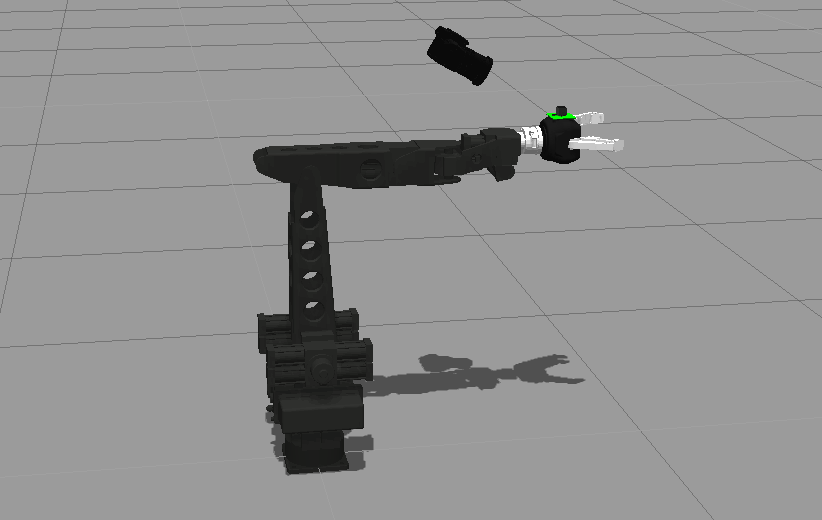
\includegraphics[scale=0.7]{Figuras/kraft-gazebo}
\caption{Representación del sistema simulado en la posición inicial de todas las simulaciones efectuadas.}
\label{fig:posinicial}
\end{figure}

La posición inicial del sistema consta de las coordenadas de la posición, $p$, de la orientación, $q$, de la velocidad lineal, $v_p$, y angular, $\omega$, del centro de masas del extremo del robot con respecto al sistema de referencia fijo, situado en la base del robot, tal y como se describió en capítulos anteriores. \par 

Las unidades en las que se miden estas magnitudes son expresadas por el Sistema Internacional de Unidades (\acrshort{si}), a saber: $m$, para posición; $m/s$, para velocidad lineal; $rad/s$, para velocidad angular y adimensional para cuaternios. \par 

Los valores concretos de la posición inicial, $\boldsymbol{x}_0$ se encuentran en la expresión (\ref{eq:posini}). El desarrollo llevado a cabo para la verificación de la observabilidad puede encontrarse en el Apéndice \ref{app:implemObservabilidad}. \par 

Para la posición inicial mostrada en la expresión (\ref{eq:posini}), se obtiene una \emph{matriz de observabilidad}, \emph{O}, de rango 13, por lo que el sistema puede ser considerado localmente observable.

\begin{equation}
	\boldsymbol{x}_0 = 
	\begin{pmatrix}
		p_x\\p_y\\p_z \\ q_0\\q_1\\q_2\\q_3 \\ v_x\\v_y\\v_z \\ \omega_x \\ \omega_y \\ \omega_z
	\end{pmatrix} =
	\begin{pmatrix}
		0\\0.5758\\0.9301 \\ 1\\0\\0\\0 \\ 0\\0\\0 \\ 0\\0\\0
	\end{pmatrix}
\label{eq:posini}
\end{equation}

\subsection{Desarrollo del observador}

Como ya se ha mencionado con anterioridad, el desarrollo del algoritmo detallado en el apartado \ref{sec:AlgoritObservador} se ha realizado en MATLAB, debido a la mayor comodidad que esto supone para el tratamiento de los datos obtenidos por los sensores, para el análisis de los resultados y por la gran cantidad de herramientas que dota este entorno. \par

Se mencionarán ciertos aspectos que es preciso remarcar acerca del desarrollo práctico del algoritmo observador y estimador de fuerzas externas descrito previamente. \par 

\subsubsection{Obtención de las propiedades físicas}

Para el correcto funcionamiento del observador, es preciso definir correctamente una serie de propiedades físicas inherentes al sistema como son la matriz de inercia, masa y vectores posición entre los distintos sistemas de referencia adoptados, expuestos en el anterior capítulo. \par 

Debido al uso del simulador \emph{Gazebo}, la obtención de estas propiedades es inmediata, puesto que es el propio sistema el que efectúa todas las operaciones necesarias para obtener esta información. \par 

Para la obtención de estos datos, es preciso llevar a cabo una doble conversión entre formatos de descripción del robot. Ésta ha sido llevada a cabo mediante el lenguaje que permite el uso de macros llamado \acrshort{xacro}, por otro lado, \acrshort{ros} emplea el formato \acrshort{urdf}, mientras que \emph{Gazebo} solamente entiende \acrshort{sdf}, por lo que es preciso realizar las siguientes conversiones:

\begin{itemize}
\item Conversión de \acrshort{xacro} a \acrshort{urdf}. De esta manera puede analizarse la descripción del robot que emplea \acrshort{ros}.
\item Conversión de \acrshort{urdf} a \acrshort{sdf}, pudiéndose ver el resultado final empleado por \emph{Gazebo} para el tratamiento del robot.
\end{itemize}

Este proceso de conversión es llevado a cabo cada vez que se lanza el simulador mediante el comando \emph{roslaunch}, pero no produce ningún fichero como resultado, por eso es preciso utilizar las instrucciones propios de \acrshort{ros} y \emph{Gazebo} para llevar a cabo estas operaciones y así poder guardar el documento resultante. \par 

Los valores de estas constantes, obtenidos directamente del fichero \acrshort{sdf} se muestran a continuación:

\[
\begin{split}
	m = 1.9603 \; [kg] \; ; \quad 
	^p\boldsymbol{r}_s = \begin{pmatrix}
		0.0125382 \\ -0.135238 \\ -0.00297882
	\end{pmatrix} \; [m] \; ; \quad 
	^p\boldsymbol{r}_E = \begin{pmatrix}
		0 \\ 0 \\ 0
	\end{pmatrix} \; [m] \\
	I_p = \begin{pmatrix}
		0.0883996 & 0.00542158 & -9.23495e^{-6} \\ 0.00542158 & 0.0575916 & -5.03661e^{-5} \\ -9.23495e^{-6} & -5.03661e^{-5} & 0.0386523
	\end{pmatrix} [kg \: m^2]
\end{split}
\]

Como ya se explicó durante la descripción del sistema simulado, el punto en el que se aplica la fuerza externa es el propio centro de masas debido a que así lo realiza el \emph{plugin} de \emph{Gazebo} desarrollado para ello, y por esta razón $^p\boldsymbol{r}_E$ es un vector nulo. \par 

Por otro lado, el valor de la estimación inicial de la posición es el mismo que el expresado en (\ref{eq:posini}).

\subsubsection{Modelado del ruido}

Uno de los aspectos más importantes a la hora de implementar un \emph{Filtro de Kalman}, o cualquiera de sus derivados, consiste en el correcto modelado del ruido existente en los sensores, incluidos en el modelo del sistema mediante las variables aleatorias $v_x$ y $v_y$, como puede apreciarse en la expresión (\ref{eq:ecObservador}). \par

Puesto que el sistema empleado para verificar la validez y efectividad del observador ha sido el simulado con \emph{Gazebo}, el ruido existente en los sensores puede ser concretado en la especificación del robot por medio de los \emph{plugins}, por lo que esta dificultad ha sido suavizada por esta situación. En el caso del sistema real hubiese sido mucho más complejo el afino del modelo del ruido. \par 

Tras diversos experimentos se ha verificado, debido a la naturaleza del \emph{Filtro de Kalman}, que al especificar ruido nulo en todos los sensores, el algoritmo no puede ejecutarse debido a la singularidad de las matrices de covarianza, lo que impide que sean invertibles, por lo que el algoritmo no es aplicable. Si se especifica una pequeña covarianza los resultados son igualmente insatisfactorios, por lo que es preciso que exista cierto orden de ruido para que el algoritmo pueda ejecutarse. \par 

La matriz de covarianzas, por mayor sencillez, se ha considerado diagonal, y con los valores de la diagonal idénticos a los especificados en la descripción del robot a la hora de definir los \emph{plugins} de los sensores. \par 

Debido a que la obtención de la aceleración angular se ha realizado derivando numéricamente la velocidad angular medida por el sensor inercial, existe una notable amplificación del ruido propia de cualquier proceso de derivación, por lo que se ha llegado a la conclusión, experimentalmente, de considerar la covarianza del ruido propio de esta variable diez veces superior al especificada para la \acrshort{imu}. \par 

\subsubsection{Acondicionamiento de datos}

Puesto que los datos obtenidos de los sensores no son directamente utilizables en el algoritmo, es preciso efectuar un proceso de modificación y acondicionamiento de los datos. Este proceso será descrito en mayor detenimiento en este apartado. \par

Como ya se explicó en este capítulo, las variables empleadas en la implantación del observador se obtienen directamente de los sensores fuerza par e inercial, como se muestra en la tabla \ref{tab:fuentevariables}. \par  

Para automatizar el proceso de acondicionamiento de los datos obtenidos se ha desarrollado un \emph{script} en MATLAB, el cual es mostrado en el apéndice \ref{app:acondicionamientoDatos}. El único dato que puede emplearse directamente sin necesidad de efectuar un procesamiento del mismo es el de la velocidad angular medida por el sensor inercial (\acrshort{imu}). \par 

A esta lista sería necesario incluir, solamente para el caso de emplear el simulador Gazebo, la obtención de la posición y orientación, puesto que es obtenida directamente del \emph{plugin} encargado de efectuar la integración de la aceleración lineal y velocidad angular (odometría). En el sistema real esta integración debe incluirse en el código del acondicionamiento de datos. \par 

A continuación se detalla las modificaciones que es necesario efectuar para la obtención de cada variable mostrada en la tabla \ref{tab:fuentevariables} que no es directamente obtenible de los sensores:

\begin{itemize}
\item $\boldsymbol{U}_S$: El sensor fuerza par mide las fuerzas y momentos que el elemento terminal ejerce sobre el sensor, $\boldsymbol{U}_S^S$, pero para emplear estos datos es necesario disponer, para que se cumplan las ecuaciones de Newton-Euler, de la fuerza que ejerce el sensor sobre el elemento terminal, $\boldsymbol{U}_S^P$. Para ello simplemente se emplea el opuesto de las fuerzas y momentos medidas por el sensor:

\[ \boldsymbol{U}_S^P = -\boldsymbol{U}_S^S \]

\item $\boldsymbol{v}_P$: El sensor inercial mide directamente aceleraciones $\boldsymbol{a}_I$, por lo que es preciso integrar numéricamente para obtener una estimación de la velocidad del sistema del acelerómetro $\boldsymbol{v}_I$:

\[ \boldsymbol{v}_{I,k} = \boldsymbol{v}_{I,k-1} + T_S \boldsymbol{a}_{I,k} \]

\noindent
siendo $T_S$ el tiempo de muestreo. Además, como se mencionó en el capítulo anterior, es preciso referir la velocidad al centro de masas mediante la expresión (\ref{eq:convVel}):

\[ \boldsymbol{v}_P = \boldsymbol{v}_I +\boldsymbol{\omega} \times \boldsymbol{^Ir_P} \]

\item $\boldsymbol{\dot{\omega}}$: El sensor inercial es capaz de medir velocidades angulares, $\boldsymbol{\omega}$, por lo que es preciso efectuar una derivación numérica para obtener la aceleración angular requerida para la implantación del observador:

\[ \boldsymbol{\dot{\omega}}_k = \frac{\boldsymbol{\omega}_k - \boldsymbol{\omega}_{k-1}}{T_S} \]

Esta derivación numérica conlleva dificultades prácticas debido al ruido del sensor, el cual es amplificado mediante el operador derivada, por lo que para un correcto funcionamiento del algoritmo es indispensable que el ruido presente en las medidas del sensor inercial no sea demasiado elevado.

\item $\boldsymbol{U}_G$: puesto que el sensor inercial empleado no es capaz de medir directamente la aceleración de la gravedad, es preciso estimarla a partir de la orientación del extremo del robot. Para ello se efectúa un cambio de base del eje z desde sistema fijo, el cual representa la dirección de la aceleración de la gravedad, al sistema móvil del centro de masas, realizando una transformación directa de cuaternio a matriz de rotación o de cambio de base del sistema fijo al móvil:

\[
	R(\boldsymbol{q}) = 
	2 \begin{pmatrix}
		q_0^2 + q_1^2 - \frac{1}{2} & q_1q_2 + q_3q_0 & q_1q_3 - q_2q_0 \\
		q_1q_2 - q_3q_0 & q_0^2 + q_2^2 - \frac{1}{2} & q_2q_3 + q_1q_0 \\
		q_1q_3 + q_2q_0 & q_2q_3 - q_1q_0 & q_0^2 + q_3^2 - \frac{1}{2}
	\end{pmatrix}
\]

cuyo desarrollo puede consultarse en \cite{beggs1983kinematics} y resultado en \cite{barrientos2007fundamentos}. Puede apreciarse que la matriz mostrada es la traspuesta de la indicada en \cite{barrientos2007fundamentos}, debido a que el cuaternio empleado representa la rotación desde sistema fijo al móvil y no al contrario. \par 

Para obtener el vector de la aceleración de la gravedad se requiere, únicamente, multiplicar dicha matriz por el vector de dirección el eje z del sistema fijo y módulo $9.8 \; m/s^2$:

\[
	\boldsymbol{U}_G = R(\boldsymbol{q}) 
		\begin{pmatrix}	0 \\ 0 \\ -9.8 \end{pmatrix}
\]

\item $\boldsymbol{a}_I$: La aceleración medida por el sensor inercial, $\boldsymbol{a}_{I,total}$, incluye la componente causada por la gravedad, por lo que es preciso anularla empleando el valor obtenido en el punto anterior:

\[ \boldsymbol{a}_I = \boldsymbol{a}_{I,total} - \boldsymbol{U}_G \]

\end{itemize}